% !TeX root = ../main.tex

\chapter{Fundamentos de comunicaciones \'opticas coherentes}
\label{cap:coherentes}

\section{Introducci\'on}
\label{sec:coh-intro}

En este cap\'itulo se re\'unen los fundamentos que utiliza el resto del trabajo. Primero
se describe la cadena óptica. Luego se explica el formato
DP-QPSK, c\'omo funciona la detecci\'on coherente y qu\'e hace el procesamiento
digital con las señales provenientes del front-end. Finalmente, se especifican las m\'etricas utilizadas, es decir la
relaci\'on entre la OSNR del balance de potencia y la relaci\'on se\~nal-ruido
en el punto de decisi\'on, el umbral HD-FEC contra el que se compara todo resultado y el EVM.

\section{El enlace \'optico coherente}
\label{sec:coh-enlace}

Un enlace \'optico coherente se separa en cuatro bloques, como muestra la
\Cref{fig:enlace-panorama}. El transmisor genera los s\'imbolos y modula la portadora con ellos. Esta se\~nal viaja a trav\'es del canal, degrad\'andose en el camino. El receptor
coherente bate la se\~nal contra un oscilador local y la lleva a banda base. El procesamiento digital tiene como objetivo deshacer estas degradaciones del canal, al igual que las provocadas por el equipo transmisor y receptor.

\begin{figure}[H]
  \centering
  \begin{tikzpicture}[
    font=\footnotesize,
    bloque/.style={draw, rounded corners=2pt, align=center,
                   minimum height=4.4em, text width=7.6em, inner sep=3pt},
    flecha/.style={-{Latex[length=2mm]}, thick}
  ]
    \node[bloque] (tx)
      {\textbf{Transmisor}\\[2pt]\scriptsize s\'imbolos, l\'aser, modulador\\[-1pt]%
       \scriptsize DP-IQ};
    \node[bloque, right=1.4em of tx] (ch)
      {\textbf{Canal LEO--GEO}\\[2pt]\scriptsize p\'erdidas, Doppler,\\[-1pt]%
       \scriptsize rotaci\'on de SOP};
    \node[bloque, right=1.4em of ch] (rx)
      {\textbf{Receptor coherente}\\[2pt]\scriptsize l\'aser LO, h\'ibrido\\[-1pt]%
       \scriptsize de \SI{90}{\degree}, ADC};
    \node[bloque, right=1.4em of rx] (dsp)
      {\textbf{DSP}\\[2pt]\scriptsize bloques\\[-1pt]%
       \scriptsize de compensaci\'on};

    \draw[flecha] (tx) -- (ch);
    \draw[flecha] (ch) -- (rx);
    \draw[flecha] (rx) -- (dsp);
  \end{tikzpicture}
  \caption[Esquema del enlace \'optico coherente]{%
    Los cuatro bloques de un enlace \'optico coherente. El canal se modela en
    el \cref{cap:canal}, el transmisor y el receptor en el
    \cref{cap:transceptor}, y el procesamiento digital en el \cref{cap:dsp}.}
  \label{fig:enlace-panorama}
\end{figure}

Cada bloque se desarrolla en detalle m\'as adelante, en el
cap\'itulo que le corresponde.

\section{Formato DP-QPSK}
\label{sec:coh-dpqpsk}

QPSK transmite dos bits por s\'imbolo en cuatro fases equiespaciadas. Con mapeo
Gray, los s\'imbolos vecinos difieren en un \'unico bit
(\cref{fig:constelacion}a), de modo que el error m\'as probable cuesta un solo
bit. La probabilidad de error de bit resulta
\begin{equation}
  \BER_{\mathrm{QPSK}} = \Qfun\!\left(\sqrt{2\,\EbNo}\right)
                       = \Qfun\!\left(\sqrt{\EsNo}\right),
  \label{eq:ber-qpsk}
\end{equation}
donde la segunda igualdad usa $E_s = 2E_b$.

\begin{figure}[H]
  \centering
  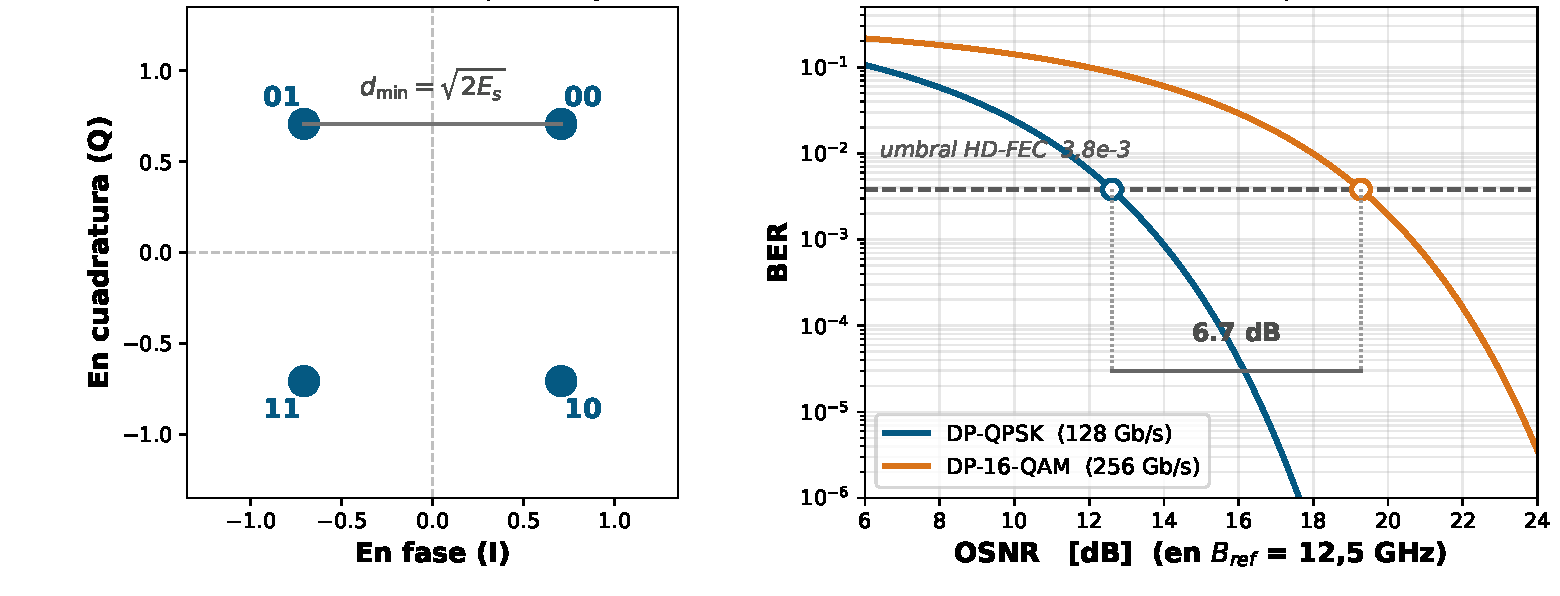
\includegraphics[width=\linewidth]{constelacion-qpsk}
  \caption[Constelaci\'on QPSK y elecci\'on del formato]{%
    (a)~Constelaci\'on QPSK con mapeo Gray. (b)~BER te\'orica contra OSNR a
    igual tasa de s\'imbolo (\SI{32}{\giga\baud}) y con las dos
    polarizaciones, para DP-QPSK y para 16-QAM. La comparaci\'on entre las dos
    se discute en la \cref{sec:coh-eleccion}.}
  \label{fig:constelacion}
\end{figure}

La multiplexaci\'on en polarizaci\'on (DP) duplica la tasa de bits sin
ensanchar el espectro, al transmitir dos secuencias QPSK independientes sobre
los dos modos ortogonales de polarizaci\'on de la misma portadora. A
\SI{32}{\giga\baud} con dos bits por s\'imbolo y dos polarizaciones se llega a
los \SI{128}{\giga\bit\per\second} de este trabajo.

Esto tiene dos costos. Por un lado, la potencia de transmisi\'on se reparte entre las dos
secuencias. Y por otro, el canal, que rota la polarizaci\'on de manera arbitraria y
variable, las mezcla, por lo que el receptor necesita un ecualizador MIMO
$2\times2$ que las vuelva a separar.

\section{Detecci\'on coherente}
\label{sec:coh-deteccion}

Para recuperar la informaci\'on de amplitud y fase presente en la portadora
\'optica hace falta un esquema de detecci\'on coherente. Un receptor de
detecci\'on directa mide $\abs{E_r}^2$, donde $E_r$ es el campo recibido, perdiendo la informaci\'on de la fase. La detecci\'on coherente consiste en hacer interferir la se\~nal recibida
contra un l\'aser oscilador local (LO) siguiendo la estructura de la
\Cref{fig:frontend}, conservando el campo completo. Como resultado, se habilitan
los formatos de modulaci\'on en amplitud y fase.

\begin{figure}[H]
  \centering
  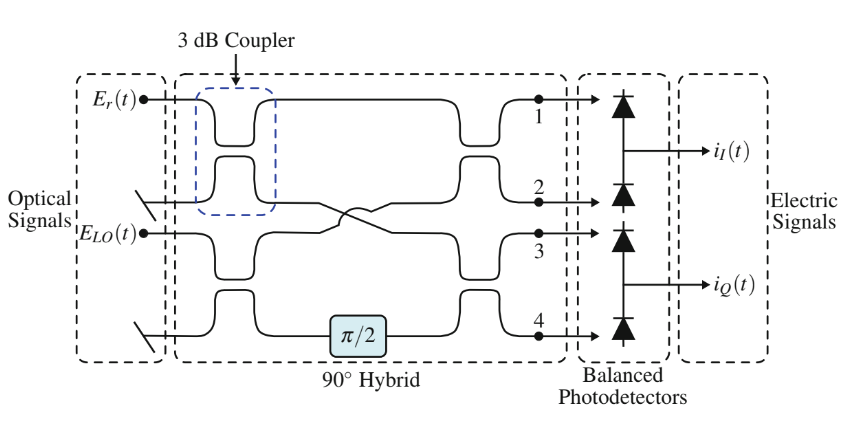
\includegraphics[width=0.86\linewidth]{FrontEndOpticoLibro}
  \caption[Front end \'optico coherente]{%
    Front end \'optico coherente de una polarizaci\'on: h\'ibrido de
    \SI{90}{\degree} formado por acopladores de \SI{3}{\dB} y dos pares de
    fotodetectores balanceados. Tomado de~\cite{mello2021}.}
  \label{fig:frontend}
\end{figure}

El bloque elemental es el acoplador de \SI{3}{\dB}, cuya matriz de
transferencia es
\begin{equation}
  \tilde{H}_c = \frac{1}{\sqrt{2}}
  \begin{bmatrix} 1 & 1 \\ 1 & -1 \end{bmatrix}.
  \label{eq:acoplador}
\end{equation}

Cuatro acopladores y un desfasaje de $\pi/2$ en una rama forman el h\'ibrido de
\SI{90}{\degree} de la \cref{fig:frontend}. Con $E_{LO}$ el campo del
oscilador local, los cuatro campos de salida resultan
\begin{equation}
  E_{1,2} = \tfrac{1}{2}\left(E_r \pm E_{LO}\right),
  \qquad
  E_{3,4} = \tfrac{1}{2}\left(E_r \pm j\,E_{LO}\right).
  \label{eq:hibrido}
\end{equation}

Cada par se detecta en configuraci\'on balanceada, es decir restando las dos
fotocorrientes,
\begin{equation}
  i_I(t) = i_1 - i_2 = R\abs{E_1}^2 - R\abs{E_2}^2,
  \qquad
  i_Q(t) = i_3 - i_4 = R\abs{E_3}^2 - R\abs{E_4}^2,
  \label{eq:balanceado}
\end{equation}
donde $R$ es la responsividad de los fotodiodos. Al utilizar fotodetectores
balanceados, los t\'erminos de detecci\'on directa $\abs{E_r}^2$ y
$\abs{E_{LO}}^2$ aparecen con el mismo signo y se cancelan, quedando
\'unicamente el batido entre se\~nal y oscilador local. Escribiendo
$E_r = A_r e^{j(\omega_s t + \phi_r)}$ y $E_{LO} = A_{LO} e^{j\omega_{LO} t}$,
\begin{align}
  i_I(t) &= A_r A_{LO} R\;\Re\!\left\{e^{\,j[\phi_r(t)+\omega_{IF}t]}\right\}
          = A_r A_{LO} R\cos\!\left(\phi_r(t)+\omega_{IF}t\right),
          \label{eq:iI}\\[2pt]
  i_Q(t) &= A_r A_{LO} R\;\Re\!\left\{e^{\,j[\phi_r(t)+\omega_{IF}t-\pi/2]}\right\}
          = A_r A_{LO} R\sin\!\left(\phi_r(t)+\omega_{IF}t\right),
          \label{eq:iQ}
\end{align}
con $\omega_{IF} = \omega_s - \omega_{LO}$ la frecuencia intermedia. Las dos
cuadraturas se combinan en una \'unica se\~nal compleja en banda base
equivalente,
\begin{equation}
  i(t) = i_I(t) + j\,i_Q(t) = R\,A_r A_{LO}\, e^{\,j[\phi_r(t)+\omega_{IF}t]},
  \label{eq:banda-base}
\end{equation}
que es la entrada del DSP luego del muestreo.

En~\eqref{eq:banda-base} se observa que la se\~nal \'util aumenta con $A_{LO}$.
Un oscilador local fuerte amplifica el batido sin amplificar el ruido
t\'ermico del amplificador de transimpedancia, de modo que el receptor, en
ausencia de un pre-amplificador \'optico, queda limitado por el ruido de
disparo del propio LO.

Cualquier desalineaci\'on entre las frecuencias de los dos l\'aseres,
incluyendo el corrimiento Doppler del enlace, aparece directamente como el
t\'ermino $\omega_{IF}t$. Es una rampa de fase que el procesamiento digital
debe estimar y eliminar antes de decidir sobre el s\'imbolo. De esa
estimaci\'on se encarga el bloque de recuperaci\'on de frecuencia, que se
desarrolla en el \cref{cap:dsp}. Su rango de captura es uno de los l\'imites
que mide el \cref{cap:tolerancias}.

\section{DSP del receptor}
\label{sec:coh-dsp-panorama}

La se\~nal que entrega el front end en la ecuaci\'on~\eqref{eq:banda-base}
tiene las cuadraturas desbalanceadas, una rampa de fase por el offset de
frecuencia, las dos polarizaciones mezcladas, y est\'a muestreada con una fase
de reloj incorrecta. El DSP deshace esas degradaciones a trav\'es de la cadena
de la \cref{fig:dsp-panorama}.

\begin{figure}[H]
  \centering
  \begin{tikzpicture}[
    font=\footnotesize,
    bloque/.style={draw, rounded corners=2pt, align=center,
                   minimum height=3.1em, text width=6.6em, inner sep=2pt},
    flecha/.style={-{Latex[length=2mm]}, thick}
  ]
    \node[bloque] (adc) {ADC\\[1pt]\scriptsize 2 muestras\\[-1pt]\scriptsize por s\'imbolo};
    \node[bloque, right=0.9em of adc]  (gsop) {Ortogonalizaci\'on\\[1pt]\scriptsize GSOP};
    \node[bloque, right=0.9em of gsop] (foc)  {Recuperaci\'on de frecuencia};
    \node[bloque, right=0.9em of foc]  (mf)   {Filtro adaptado\\[1pt]\scriptsize RRC};

    \node[bloque, below=3.0em of adc]  (clk)  {Recuperaci\'on de reloj};
    \node[bloque, right=0.9em of clk]  (eq)   {Ecualizador MIMO $2\times2$\\[1pt]\scriptsize DDLMS};
    \node[bloque, right=0.9em of eq]   (cpr)  {Recuperaci\'on de fase};
    \node[bloque, right=0.9em of cpr]  (dec)  {Decisi\'on\\[1pt]\scriptsize EVM y BER};

    \draw[flecha] (adc)  -- (gsop);
    \draw[flecha] (gsop) -- (foc);
    \draw[flecha] (foc)  -- (mf);
    \draw[flecha] (clk)  -- (eq);
    \draw[flecha] (eq)   -- (cpr);
    \draw[flecha] (cpr)  -- (dec);

    \coordinate (bajada) at ($(mf.south)+(0,-1.05em)$);
    \draw[flecha] (mf.south) -- (bajada) -| (clk.north);
  \end{tikzpicture}
  \caption[Cadena de procesamiento digital del receptor]{%
    DSP. En la implementaci\'on de este trabajo el ecualizador MIMO y la
    recuperaci\'on de fase est\'an integrados. Son dos lazos adaptativos
    distintos que operan sobre las mismas muestras.}
  \label{fig:dsp-panorama}
\end{figure}

Cada bloque se encarga de una degradaci\'on concreta:

\begin{itemize}\itemsep2pt
  \item \textbf{Ortogonalizaci\'on (GSOP):} Se encarga de corregir el
        desbalance de ganancia y de cuadratura entre las componentes I y Q que
        introducen el h\'ibrido y los fotodetectores.
  \item \textbf{Recuperaci\'on de frecuencia:} Estima y quita el t\'ermino
        $\omega_{IF}$ de la ecuaci\'on~\eqref{eq:banda-base}, que en este
        enlace est\'a dominado por el Doppler.
  \item \textbf{Filtro adaptado:} Aplica la mitad del coseno alzado que falta
        para completar el criterio de Nyquist y maximizar la relaci\'on
        se\~nal-ruido en el instante de muestreo.
  \item \textbf{Recuperaci\'on de reloj:} Corrige el error de frecuencia y de
        fase de muestreo respecto del reloj del transmisor.
  \item \textbf{Ecualizador MIMO $2\times2$:} Invierte la matriz de Jones del
        canal y separa las dos polarizaciones. Sigue adem\'as su rotaci\'on a
        lo largo del pase.
  \item \textbf{Recuperaci\'on de fase:} Cancela el ruido de fase de los
        l\'aseres y el error de frecuencia residual.
  \item \textbf{Decisi\'on:} Mapea cada s\'imbolo al punto m\'as cercano de la
        constelaci\'on, y calcula EVM y BER.
\end{itemize}

La implementaci\'on de cada bloque, con sus par\'ametros y sus l\'imites de
operaci\'on, se desarrolla en el \cref{cap:dsp}.

\section{M\'etricas de desempe\~no}
\label{sec:coh-metricas}

\subsection{OSNR y relaci\'on se\~nal-ruido}
\label{sec:coh-osnr}

El balance de potencia del enlace se expresa en OSNR, medida en un ancho de
banda de referencia convencional $\Bref = \SI{12.5}{\giga\hertz}$
(\SI{0.1}{\nano\metre} en banda C). La detecci\'on, en cambio, depende de la
relaci\'on se\~nal-ruido. La conversi\'on entre ambas es
\begin{equation}
  \EsNo\,[\si{\dB}] = \OSNR\,[\si{\dB}] + 10\log_{10}\!\frac{\Bref}{\Rs}.
  \label{eq:osnr-esno}
\end{equation}
A \SI{32}{\giga\baud} el segundo t\'ermino vale \SI{-4.08}{\dB}.

La diferencia entre las dos es el ancho de banda sobre el que se integra el
ruido. El de referencia est\'a fijo, mientras que el del punto de decisi\'on sigue a la
tasa de s\'imbolo. Por eso la OSNR describe al canal y la relaci\'on
se\~nal-ruido describe lo que necesita el receptor.

\subsection{El umbral HD-FEC}
\label{sec:coh-fec}

Los sistemas de comunicaciones se dise\~nan para operar por debajo de un umbral
pre-FEC que un c\'odigo de correcci\'on posterior lleva a una BER de salida
mucho m\'as baja. Este trabajo adopta el umbral cl\'asico de decisi\'on dura
(HD-FEC) con \SI{7}{\percent} de \emph{overhead},
$\BER = 3{,}8\times10^{-3}$, correspondiente al c\'odigo de bloque del
ap\'endice~I.9 de la recomendaci\'on ITU-T G.975.1~\cite{itu_g975}, que lleva
la entrada a una tasa de errores de menos de $10^{-13}$ a la salida.

Combinando \eqref{eq:ber-qpsk} y \eqref{eq:osnr-esno}, ese umbral requiere
$\EbNo = \SI{5.52}{\dB}$, equivalente a $\EsNo = \SI{8.53}{\dB}$ y a
$\OSNR = \SI{12.61}{\dB}$ te\'oricos. Este valor es el punto de comparaci\'on
de todos los barridos del \cref{cap:tolerancias}. La diferencia entre la OSNR
simulada y los \SI{12.61}{\dB} es la penalidad de implementaci\'on del
receptor.

Adoptar un umbral fijo permite reducir todo el desempe\~no del enlace a una
sola pregunta binaria por cada condici\'on de canal. Si la BER pre-FEC queda
por debajo de $3{,}8\times10^{-3}$, entonces el sistema funciona.

\subsection{Estimaci\'on de la BER mediante el EVM}
\label{sec:coh-evm}

La magnitud del vector de error (EVM) mide la dispersi\'on de los s\'imbolos
recibidos alrededor de sus posiciones ideales. Se define como la ra\'iz del
error cuadr\'atico medio respecto de la referencia, normalizado a la potencia
media de la constelaci\'on,
\begin{equation}
  \EVM = \sqrt{\frac{\E{\abs{r_k - s_k}^2}}{\E{\abs{s_k}^2}}},
  \label{eq:evm}
\end{equation}
donde $r_k$ es el s\'imbolo recibido y $s_k$ el transmitido.

Para una constelaci\'on de energ\'ia constante como QPSK, y bajo la
hip\'otesis de ruido gaussiano complejo, el EVM es directamente el inverso de
la ra\'iz de la relaci\'on se\~nal-ruido, y la BER se estima como
\begin{equation}
  \EVM_{\mathrm{rms}}^{2} \simeq \frac{1}{\mathrm{SNR}},
  \qquad
  \BER \simeq \Qfun\!\left(\frac{1}{\EVM_{\mathrm{rms}}}\right).
  \label{eq:evm-ber}
\end{equation}

La consistencia de \eqref{eq:evm-ber} con el umbral HD-FEC se comprueba
directamente, ya que $\Qfun(1/0{,}3746) = 3{,}80\times10^{-3}$. Es decir,
$\EVM = \SI{37.46}{\percent}$ es el umbral HD-FEC expresado como EVM, y las dos
m\'etricas son intercambiables mientras el ruido dominante sea gaussiano.



\subsection{Estimaci\'on de la BER por conteo de errores}
\label{sec:coh-conteo}

La BER contada tiene un piso que no depende del receptor sino del largo de la
simulaci\'on. Si sobre $N$ bits no se observa ning\'un error, la regla de tres
establece que el intervalo de confianza del \SI{95}{\percent} para la
probabilidad de error tiene cota superior
\begin{equation}
  \BER_{\min} = \frac{3}{N}.
  \label{eq:piso-conteo}
\end{equation}
Con $N_{\mathrm{symb}} = 3\times10^{5}$ s\'imbolos por polarizaci\'on, el piso
est\'a en el orden de $5\times10^{-6}$, lo que implica una cota m\'axima de
OSNR que se puede analizar.

El EVM no tiene este problema. Se calcula sobre todos los s\'imbolos, converge
con un n\'umero mucho menor de ellos y var\'ia de forma continua incluso donde
no hay errores. Por eso, en los barridos de tolerancia del
\cref{cap:tolerancias} la m\'etrica principal es el EVM y la BER que se reporta
es la estimada mediante \eqref{eq:evm-ber}. La BER contada se usa solo como
verificaci\'on, donde el n\'umero de errores es estad\'isticamente suficiente.

\section{Elecci\'on del formato}
\label{sec:coh-eleccion}

La alternativa para duplicar la tasa de bits es subir el orden de la
modulaci\'on en lugar de multiplexar en polarizaci\'on. Con las m\'etricas ya
definidas, las dos opciones se pueden comparar sobre el mismo eje. La
\cref{fig:constelacion}b muestra por qu\'e no se eligi\'o este camino.

A igual tasa de s\'imbolo, 16-QAM entrega \SI{256}{\giga\bit\per\second} pero
necesita \SI{19.3}{\dB} de OSNR para alcanzar el umbral HD-FEC, frente a los
\SI{12.6}{\dB} de DP-QPSK. Son \SI{6.7}{\dB} adicionales, o \SI{3.7}{\dB} si la
comparaci\'on se hace a igual tasa de bits, que un enlace limitado
por potencia puede ahorrarse.

Hay una segunda raz\'on. Al tener una separaci\'on angular menor y un nivel
m\'as en amplitud que QPSK, 16-QAM es bastante m\'as sensible al ruido de fase
y al RIN de los l\'aseres. DP-QPSK es entonces el formato que maximiza la tasa
de bits dentro del presupuesto de potencia disponible.

\section{Conclusiones}
\label{sec:coh-conclusiones}

El enlace se separa en transmisor, canal, receptor coherente y procesamiento
digital. Este cap\'itulo describi\'o los cuatro bloques a grandes rasgos, y cada uno
se retoma despu\'es en su propio cap\'itulo.

Con detecci\'on coherente se obtiene la informaci\'on de fase y de amplitud del
campo en banda base equivalente, ecuaci\'on~\eqref{eq:banda-base}, y con ella
la posibilidad de modular en amplitud, fase y polarizaci\'on. El precio es que
toda desalineaci\'on entre los dos l\'aseres queda integrada en la se\~nal como
una rampa de fase que el DSP debe deshacer.

El desempe\~no se reporta contra un \'unico umbral,
$\BER = 3{,}8\times10^{-3}$, equivalente a $\OSNR = \SI{12.61}{\dB}$
te\'oricos y a $\EVM = \SI{37.46}{\percent}$. La m\'etrica principal de los
barridos es el EVM, porque no tiene el piso de conteo $3/N$ que limita a la BER
por conteo de errores.

En base a este umbral, la tasa de \SI{32}{\giga\baud} con DP-QPSK es el punto de operaci\'on que
maximiza la tasa de bits dentro del presupuesto de potencia disponible.